\documentclass[conference]{IEEEtran}
\pagenumbering{roman}
\input ./common-macros.tex
\IEEEoverridecommandlockouts
% The preceding line is only needed to identify funding in the first footnote. If that is unneeded, please comment it out.
\usepackage{cite}
\usepackage{algorithmic}
\usepackage{graphicx}
\usepackage{textcomp}
\usepackage{xcolor}
\usepackage{CJK}
\usepackage{amsfonts, mathrsfs, bm, amsmath, mathabx, amssymb}
\usepackage[margin=1cm]{geometry}
\usepackage{minted}
\usepackage{array}
\usepackage{makecell}
\usepackage{url}
\def\BibTeX{{\rm B\kern-.05em{\sc i\kern-.025em b}\kern-.08em
    T\kern-.1667em\lower.7ex\hbox{E}\kern-.125emX}}

\begin{document}
\begin{CJK}{UTF8}{bkai}

\title{論演唱會抽票賽局中的邊際效益遞減現象}

\author{\IEEEauthorblockN{李丞恩}}

\maketitle

\begin{abstract}
本文考慮一個抽票賽局模型,其中每位參與者購買至少一張 CD 並獲得相應的抽獎券,最終依據抽獎機制決定中獎結果。本文從單一參與者的角度與賽局互動下,分別探討中獎機率、效用/投資比的最佳選擇以及納許均衡解。透過數學推導與數值模擬,本文揭示了在獨立最佳策略下最佳購買數與在納許均衡下過度投入之間的顯著差異,進而呈現出邊際效益遞減與競爭過度投入的現象。
\end{abstract}

\begin{IEEEkeywords}
抽票賽局, 邊際效益, 納許均衡, 冪定律, 賽局理論
\end{IEEEkeywords}

\bsec{前言}{intro}

在現代演唱會及各類抽獎活動中,參與者通常會透過購買多張 CD 或票券來提高中獎機率,但由於每人最多只能中獎一次,這種策略可能導致邊際效益遞減。本文旨在利用賽局理論方法構建一個抽票賽局模型,分析個體在成本效用平衡下的獨立最佳策略與考慮其他參與者行為後的納許均衡策略之間的差異。

\bsec{問題定義}{Definition}

設共有 $N$ 個人參與,總共購買 $M$ 張 CD(每人至少一張,且 $M>N$),每張 CD 附帶一張抽獎券。若總獎品數為 $K$ 且每人最多中獎一次,抽獎過程定義如下:
\begin{enumerate}
    \item 每位參與者購買 $n_i$ 張 CD,滿足 $\sum_{i=1}^{N} n_i=M$。
    \item 若 $K \ge N$,則所有人均中獎。
    \item 若 $K<N$,則從 $M$ 張抽獎券中以等機率(每張機率 $1/M$)依次抽出一張。若抽出的券屬於第 $i$ 人,則該人中獎,並將其所有券從獎池中移除。
    \item 重複直至$K$個獎品全數抽出。
\end{enumerate}

\bsubsec{單一參與者的中獎機率}{2-1}

由於抽選最終的結果僅決定於哪幾位參與者的票券至少被抽出一次,因此該抽獎機制等價於從所有 $M$ 張抽獎券中隨機抽取 $K$ 張後不放回,若某人至少有一張券被抽到則中獎\footnote{如果一個人有多張被抽中,最終仍只算一次得獎}。這是因為對於參與者 $i$ 來說,其是否中獎完全取決於在這 $K$ 張中是否至少有一張屬於 $i$。

因此,對於第 $i$ 個人,其中獎機率可表示為:
\bear{win_prob}
    p_i &=& 1 - \Pr(\text{其所有 } n_i \text{ 張券均不在 } K \text{ 張中})\\
    &=&1 - \frac{\binom{M-n_i}{K}}{\binom{M}{K}}.
\eear
明顯地,當 $n_i$ 增大時,分子 $\binom{M-n_i}{K}$ 變小,因此 $p_i$隨 $n_i$ 嚴格單調遞增。

\bsubsec{在成本考量下最佳「投資」(票數)選擇}{2-2}

假設每張 CD 價格為 $c$,而額外存在一筆固定成本 $d>0$(或可以看作是「進入成本」)\footnote{例如獎品為演唱會門票的購買權時,$d$ 即為門票的票價},則一個人購買 $n_i$ 張 CD 的總成本為
\beq{cost}
    \text{Cost} = c\,n_i + d.
\eeq

考慮效用/投資比
\beq{utility}
    U(n_i) = \frac{p_i}{c\,n_i + d} = \frac{1 - \dfrac{\binom{M-n_i}{K}}{\binom{M}{K}}}{c\,n_i + d}.
\eeq
由\req{win_prob}可知 $p_i$ 隨 $n_i$ 單調上升,但同時成本線性上升,因此最佳的 $n_i$ 必須在邊際效益和邊際成本之間取得平衡。可將 $n_i$ 看作連續變數,令 $U(n_i)$ 取對數後微分等於零\footnote{取對數不改極值位置},即要求:
\bear{logU}
    \frac{d}{dn_i}\ln\Bigl(1 - \frac{\binom{M-n_i}{K}}{\binom{M}{K}}\Bigr)
    &=& \frac{d}{dn_i}\ln(c\,n_i+d)\\
    &=& \frac{c}{c\,n_i+d}\,
\eear
令 $p_i = 1 - Q(n_i)$ 其中
\bear{Qni}
    Q(n_i)&=& \frac{\binom{M-n_i}{K}}{\binom{M}{K}}\\
    &=& \prod_{j=0}^{K-1} \frac{M-n_i-j}{M-j},
\eear
所以有
\bear{diff_Q}
    \frac{d}{dn_i}\ln\bigl(1-Q(n_i)\bigr) &=& \frac{Q(n_i)}{1-Q(n_i)} \cdot \Bigl(-\frac{d}{dn_i}\ln Q(n_i)\Bigr)\\
    &=&-\sum_{j=0}^{K-1}\frac{1}{M-n_i-j}
\eear
因此,最優 $n_i$ 應滿足方程式:
\beq{optimal_ni}
    \frac{Q(n_i)}{1-Q(n_i)} \sum_{j=0}^{K-1}\frac{1}{M-n_i-j} \;=\; \frac{c}{c\,n_i+d}\,.
\eeq
其中 $M$ 往往包含其他人的購買量,如果把其他人購買數記作 $m$(即令 $M = m+n_i$ ),那麼上述條件可改寫成針對單一參與者在固定他人行為下的最佳回應。此外由於方程通常無閉合解,最終最佳的 $n_i$ 需要數值求解或進一步近似。

\bsubsec{在 $f(x)$ 為冪定律下的最佳選擇}{2-3}

假設每個人購買抽獎券數量的機率質量函數遵從冪定律,
\beq{power_law}
    f(x) \propto x^{-\gamma}\quad (\gamma>1),
\eeq
意味著在群體中出現大額購買(大 $n$ )的可能性雖然較低,但分布尾部較重。

在「他人行為給定」的情況下,令其他人購買數總和為 $m$ ,則對於第 $i$ 人,將 $M = m+n_i$ 代入\req{win_prob}得到
\beq{pi_m}
    p_i = 1 - \frac{\binom{m}{K}}{\binom{m+n_i}{K}}.
\eeq
如果假設 $m$相對較大、且 $n_i$不是太大,可利用如下近似:
\beq{comb_approx}
    \binom{m+n_i}{K} \approx \binom{m}{K}\left(1+\frac{n_i}{m}\right)^K,
\eeq
從而有
\beq{pi_approx}
    p_i \approx 1 - \left(1+\frac{n_i}{m}\right)^{-K} \;=\; 1 - \left(\frac{m}{m+n_i}\right)^K.
\eeq
將此結果代入\req{utility}此時,我需要最大化
\beq{Uni_approx}
    U(n_i) = \frac{1-\Bigl(\frac{m}{m+n_i}\Bigr)^K}{c\,n_i+d}\,.
\eeq
與前述類似,取對數後微分可得一階條件:
\beq{condition}
    \frac{K\,\frac{m}{m+n_i}\,\frac{1}{m+n_i}}{1-\Bigl(\frac{m}{m+n_i}\Bigr)^K} = \frac{c}{c\,n_i+d}\,,
\eeq
或
\beq{condition2}
    \frac{K\,m^K}{(m+n_i)^{K+1}\Bigl[1-\Bigl(\frac{m}{m+n_i}\Bigr)^K\Bigr]} = \frac{c}{c\,n_i+d}\,.
\eeq

方程式 \req{condition2} 刻畫了在冪定律分布背景下最佳購買數 $n_i^*$的隱含關係。雖然一般情況下無法寫出解析解,但可發現:
\begin{enumerate}
    \item 當成本 $c$較高或固定成本 $d$較大時,邊際獲勝率提升有限,最佳 $n_i^*$ 會趨於較低值;
    \item 當獎品數 $K$ 較大(或其他人普遍買少)時,額外購買券帶來的中獎機率增幅較明顯,則最佳 $n_i^*$ 較大。
\end{enumerate}

\bsubsec{賽局中的納許均衡}{2-4}

現在假設每個CD的購買者(在賽局理論中稱為「玩家」)都是理性決策者,均根據自己的成本與中獎機率考慮如何選擇購買數量,而全體玩家的決策共同決定 $M=\sum_{j=1}^N n_j$ 及每個人的中獎機率。令每個人的效用(或利益/成本比)為
\beq{utility_minus_i}
    U_i(n_i, n_{-i}) = \frac{p_i(n_i, n_{-i})}{c\,n_i+d}\,,
\eeq
其中$p_i(n_i, n_{-i})$由\req{win_prob}給出,代表第 $i$ 人的中獎機率
\beq{win_prob_minus_i}
    p_i(n_i, n_{-i}) = 1 - \frac{\binom{M-n_i}{K}}{\binom{M}{K}},\quad M = n_i+\sum_{j\neq i} n_j.
\eeq
在納許均衡 (Nash equilibrium) 中,對每個玩家 $i$而言,給定其他人 $n_{-i}$ 的策略,自己無法通過改變 $n_i$ 來提高 $U_i$ 。

在達到納許均衡時對稱均衡假設下\footnote{即所有玩家採取相同策略 $n^*$},此時 $M=N\,n^*$ ,而
\beq{pi_nstar}
    p_i(n^*) = 1 - \frac{\binom{(N-1)n^*}{K}}{\binom{Nn^*}{K}}\,.
\eeq
玩家的最佳回應條件(若將 $n_i$當作連續變量)要求:
\beq{react}
    \frac{d}{dn_i}\ln\Bigl(1 - \frac{\binom{M-n_i}{K}}{\binom{M}{K}}\Bigr)\Big|_{n_i=n^*} = \frac{c}{c\,n^*+d}\,.
\eeq
也就是說,對稱納許均衡 $n^*$需滿足:
\beq{Q_nash}
    \frac{Q(n^*)}{1-Q(n^*)}\sum_{j=0}^{K-1}\frac{1}{N\,n^*-n^* -j} \;=\; \frac{c}{c\,n^*+d}\,,
\eeq
其中
\beq{Q_nstar}
    Q(n^*) = \frac{\binom{(N-1)n^*}{K}}{\binom{Nn^*}{K}}\,.
\eeq
這個隱含方程決定了對稱均衡下的最佳購買數 $n^*$。

\bsec{數值分析}{Validation}

本節中我以Aqours Finale Live\cite{Aqours_finale}為例。假設只進行一次抽選,且抽選方法由\rsec{Definition}所描述的方法給出。由抽選所需的唱片銷量\cite{sales}以及\cite{Aqours_finale}給出的抽選截止日期,取 $M=303,835$。另外,取西武巨蛋\cite{dome}的座位數為 $K$ 值,$K=40,000$。

\bsubsec{估計參與者數$N$}{3-1}

假設每個人購買的 CD 數量 $n$ 服從從 1 到 100 的冪定律分布\req{power_law},
\beq{power_law_CD}
    f(n)=\frac{n^{-\gamma}}{\sum_{j=1}^{100}j^{-\gamma}},
\eeq
則平均購買數為
\beq{expected}
    E[n]=\frac{\sum_{n=1}^{100}n\;n^{-\gamma}}{\sum_{n=1}^{100}n^{-\gamma}}.
\eeq
由於總票數 $M=303,835$(單位:個),因此參與者數約可估計為
\beq{N_approx}
    N\approx\frac{M}{E[n]}.
\eeq
例如,若採用 $\gamma=2, 2.2, 2.4, 2.6, 2.8, 3$,則利用 $1\leq n\leq100$ 做截斷後,可得到:\footnote{$\gamma=2$ 時若無截斷則期望發散,因此此處採用 1~100 的截斷;數值僅為近似估計。}

\begin{table}[h]
    \centering
    \caption{不同 $\gamma$ 值下的平均購買數 $E[n]$ 與估計參與者數 $N$}
    \label{tab:gamma_estimation}
    \begin{tabular}{|c|c|c|}
        \hline
        $\gamma$ & $E[n]$ (近似) & 估計參與者數 $N$ \\
        \hline
        2.0  & 3.17  & 95,764  \\
        2.2  & 2.42  & 125,416 \\
        2.4  & 1.96  & 154,963 \\
        2.6  & 1.67  & 181,818 \\
        2.8  & 1.48  & 204,678 \\
        3.0  & 1.36  & 223,373 \\
        \hline
    \end{tabular}
\end{table}

\bsubsec{中獎機率 $p_i$ 與效用/投資比 $U(n_i)$}{3-2}

方程式\req{win_prob}給出某人中獎機率為  
\beq{win_prob2}
    p_i=1-\frac{\binom{303,835-n_i}{40,000}}{\binom{303,835}{40,000}}\,. 
\eeq
這個公式不含 $N$ 也不直接依賴於分布參數 $\gamma$。可繪製$p_i$對$n_i$的關係圖如下:

\begin{figure}[!t]
    \centering
    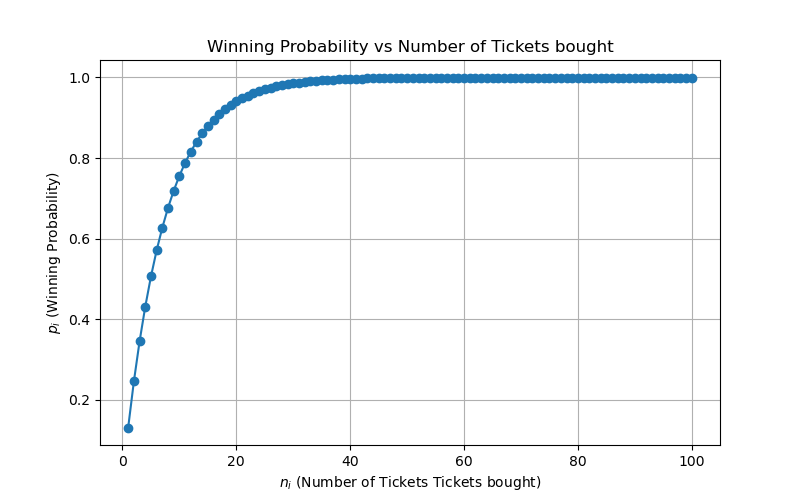
\includegraphics[width=3.45in]{probability.png}
    \caption{$p_i$對$n_i$的關係圖} %請填入
    \label{fig:probability}
\end{figure}

根據相關CD的售價以及演唱會的票價\cite{Aqours_finale},可設$c=1,650$ 日圓、$d=13,935$ 日圓。則效用/投資比定義為  
\beq{utility_val}
    U(n_i)=\frac{p_i}{1,650\,n_i+13,935}\,.
\eeq
其中 $p_i$ 由\req{utility_val}給出。其中取 $n_i=1,2,\dots,100$ 計算並作圖,

\begin{figure}[!t]
    \centering
    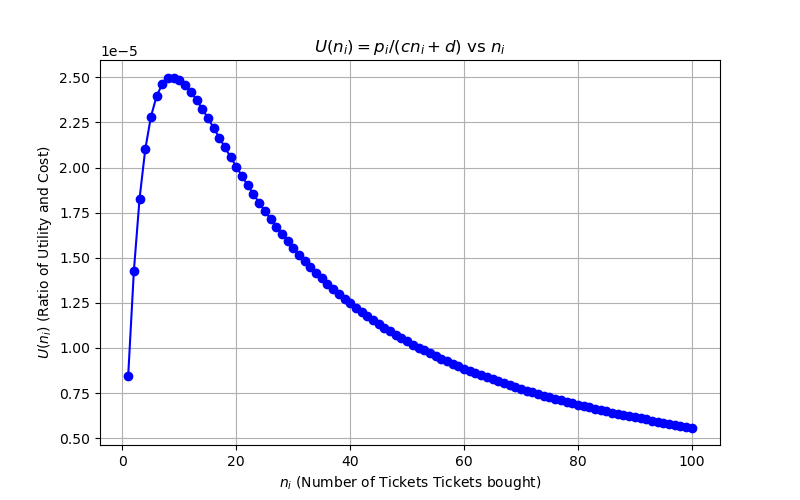
\includegraphics[width=3.45in]{utility.png}
    \caption{效用函數 $U(n_i)$ 對 $n_i$ 作圖,可發現明顯的邊際效應遞減現象} %請填入
    \label{fig:utility_fig}
\end{figure}

由\rfig{utility_fig}可知無論 $N$ 與 $\gamma$ 為何,獨立最佳化下的最佳$n_i=9$。

\bsubsec{納許均衡}{3-2} 

若所有人都採取相同策略 $n^*$,則總票數為 $M=N\,n^*$,$N$ 可用\req{N_approx}估計。而若某玩家偏離購買 $n$ 張,則假設其他人均按照原分布購買(平均值約為截斷分布的 $E[n]$),該玩家的「偏離」中獎機率可近似寫為  
\beq{p_dev}
    p_{\text{dev}}(n)=1-\frac{\binom{(N-1)E[n]}{K}}{\binom{(N-1)E[n]+n}{K}}\,.
\eeq
「偏離」後的效用為
\beq{U_dev}
    U_{\text{dev}}(n)=\frac{p_{\text{dev}}(n)}{c\,n+d}
\eeq
對稱納許均衡要求若其他人均採 $E[n]$(或在均衡下 $n^*$),則最佳回應應滿足 
\beq{nash_eq_n}
    n^*=\operatorname*{arg\,max}_n\, U_{\text{dev}}(n)
\eeq

用固定點迭代找出最佳回應$n^*$,我假設其他人依截斷分布(平均值 $E[n]$)購買,然後找出使得偏離效用最大化的 $n^*$;當對\req{U_dev}進行迭代而收斂時,所得的 $n^*$ 就是對稱納許均衡下的最佳投資決策。由此可得下表

\begin{table}[h]
    \centering
    \caption{納許均衡(對稱均衡)下的最佳投資決策}
    \label{tab:nash_equilibrium}
    \begin{tabular}{|c|c|c|}
        \hline
        $\gamma$ & 估計參與者數 $N$ & 納許均衡 $n_i^*$ \\
        \hline
        2.0  & 95,764  & 34 \\
        2.2  & 125,415 & 47 \\
        2.4  & 154,962 & 59 \\
        2.6  & 181,818 & 71 \\
        2.8  & 204,677 & 80 \\
        3.0  & 223,373 & 88 \\
        \hline
    \end{tabular}
\end{table}

\bsubsec{小結}{3-3}

當單個參與者僅考慮自身的效用/成本比,則其最佳策略由下式決定:
\beq{U_ni3}
    U(n_i)=\frac{1-\frac{\binom{M-n_i}{K}}{\binom{M}{K}}}{c\,n_i+d}\,.
\eeq
此公式僅涉及個人購買數 \(n_i\) 及固定參數 \(M, K, c, d\),而不依賴於市場參與者數量 \(N\) 或購買行為的冪定律分布參數 \(\gamma\)。因此,在所有情況下,獨立最適策略均為 9 張。

\subsubsection*{納許均衡下的最佳策略(遠大於 9 張)}
在納許均衡中,每位玩家的決策不僅取決於自身效用/成本比,還受其他參與者行為影響。當參與者數 \(N\) 增加(由冪定律截斷分布決定),市場競爭愈發激烈,導致低投入策略(如 9 張)難以維持相對優勢。

由於總票數 \(M\) 固定,當多數玩家僅投入 9 張時,個別玩家可透過增加購買量顯著提升中獎機率,形成「競爭性過度投入」現象。此「爭先」效應促使均衡策略遠高於 9 張,且隨 \(\gamma\)(及相應 \(N\))增長而進一步提高。

\begin{enumerate}
    \item 個體最佳策略(9 張)平衡了效用與成本,適用於不考慮市場互動的情境。
    \item 然而,市場競爭促使玩家提高購買數量,以避免被他人壓制。結果顯示,在納許均衡下,最佳策略介於 34 至 88 張之間。
    \item 這突顯了賽局理論中的「策略相互依賴」現象,即個體最優與均衡解可能存在顯著落差。在競爭環境中,個人為維持相對優勢會過度投入,最終導致均衡解偏離社會最優。
\end{enumerate}

總結而言,在競爭性抽獎賽局中,玩家為了確保自身優勢,最終均採取更高的投入策略,這即為「賽局均衡」效應的體現。

\bsec{結論}{Conclusion}
本文從數學模型與數值模擬角度分析了抽票賽局中的邊際效益遞減現象。結果表明當考慮參與者購買數服從冪定律分布時,市場參與者數可由截斷平均值估計,不同 $\gamma$ 值下估計結果存在差異;在賽局互動下(納許均衡),為了相對優勢,玩家往往必須投入顯著多於 9 張的票數,其均衡解隨市場參與者數增加而上升。而對於無法承受大量投入的玩家而言,獨立最佳策略(9 張)仍是其相對保守的選擇,但這將使其在競爭中處於劣勢,形成市場分層現象。

\bibliographystyle{IEEEtran}
\begin{thebibliography}{10}

\bibitem{sales}
``Love Live!'' 唱片銷量資料, \textit{atwiki}, 
\url{https://w.atwiki.jp/keroro00innovator/pages/6271.html}.

\bibitem{Aqours_finale}
Aqours Finale Live 官方網站, \textit{Love Live! Official Website}, 
\url{https://www.lovelive-anime.jp/uranohoshi/live/live_detail.php?p=Aqours_Finale}.

\bibitem{dome}
Belluna Dome (西武巨蛋), \textit{Wikipedia}, 
\url{https://en.wikipedia.org/wiki/Belluna_Dome}.

\end{thebibliography}

\end{CJK}
\end{document}
